\section{Q4} 

\subsection{Introduction} \label{sec:Introduction}

In modern automation systems, the integration of electromagnetic and electropneumatic technologies offers versatile 
and efficient solutions for controlling complex mechanical processes. This report addresses the development 
of an automatism for a double elevator system, designed to operate between two levels (floor 0 and floor 1),
as specified in Question 4 of the lab assignment. The system is modeled using single-action and double-action 
pneumatic cylinders to simulate elevator motion, with sensors and actuators coordinated through a Grafcet-based 
control logic. The objective is to ensure synchronized and reliable movement of both elevators, optimizing their 
interaction and safety through appropriate control sequences. The process is simulated and validated using FluidSIM 
3.6, providing insight into the behavior and robustness of the designed control system.

\subsection{Process Schematic and Sensor-Actuator Integration} \label{sec:Process_Schematic_and_Sensor-Actuator_Integration}

\begin{figure}[H]
    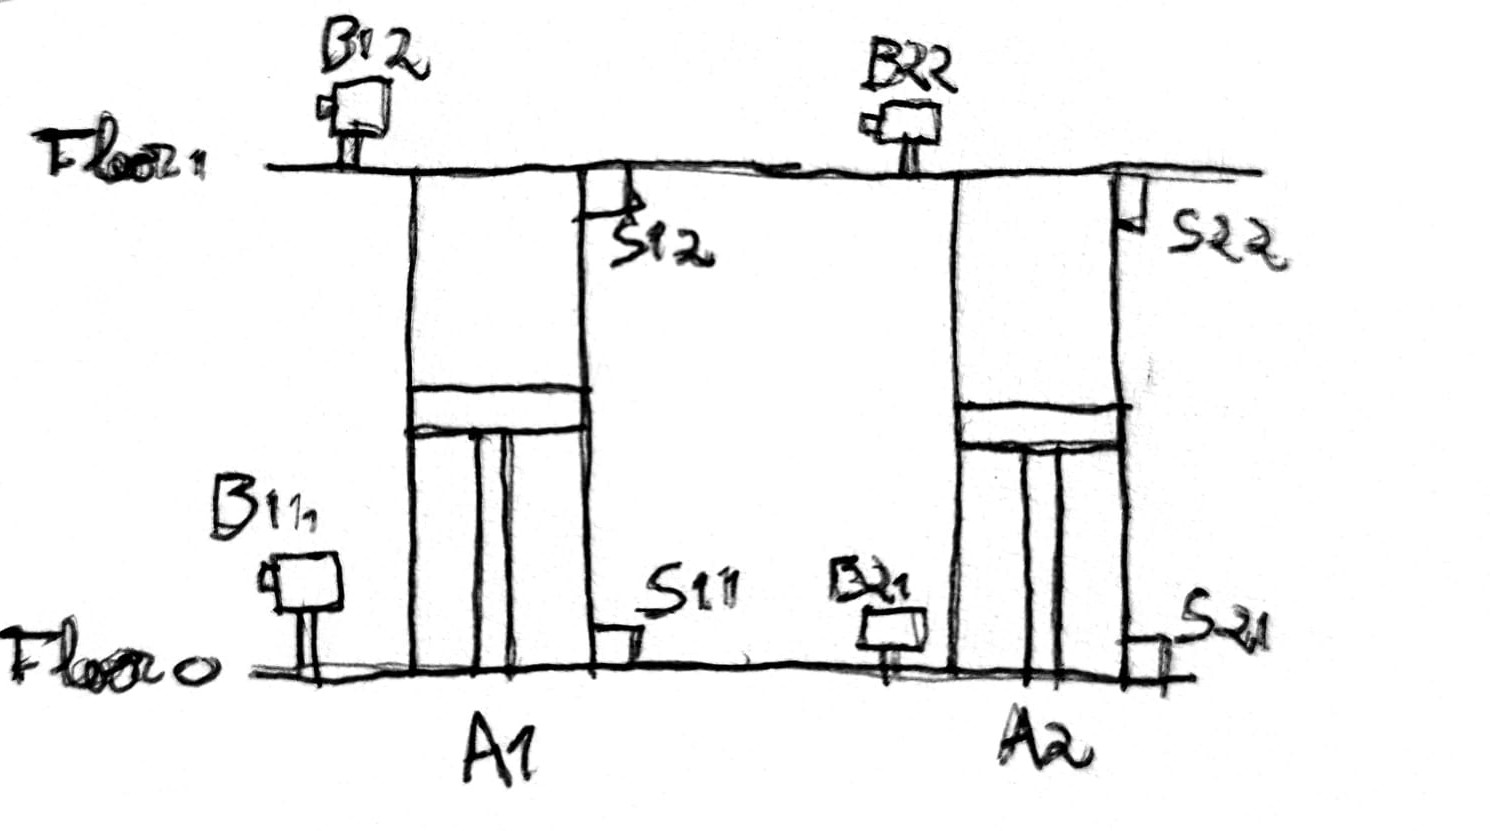
\includegraphics[width=16cm]{Images/Q4/Q4_schem.jpeg}
    \centering
    \caption{Process Schematic for Q4 system}
    \label{fig:Q4_schem}
\end{figure}

\subsection{Grafcet Representation} \label{sec:Grafcet_Representation}

\begin{figure}[H]
    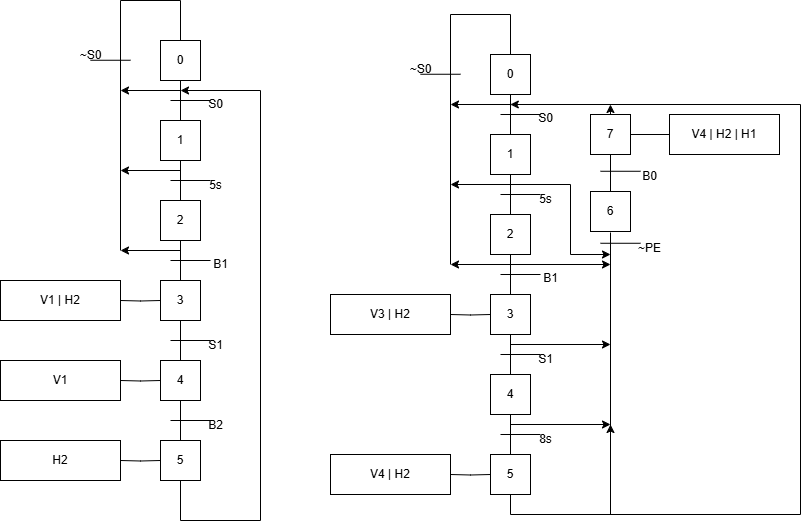
\includegraphics[width=16cm]{Images/Q4/graftset.png}
    \centering
    \caption{Grafset of the double elevator}
    \label{fig:grafset}
\end{figure}

\subsection{Simulation and Validation} \label{sec:Simulation_and_Validation}

\begin{figure}[H]
    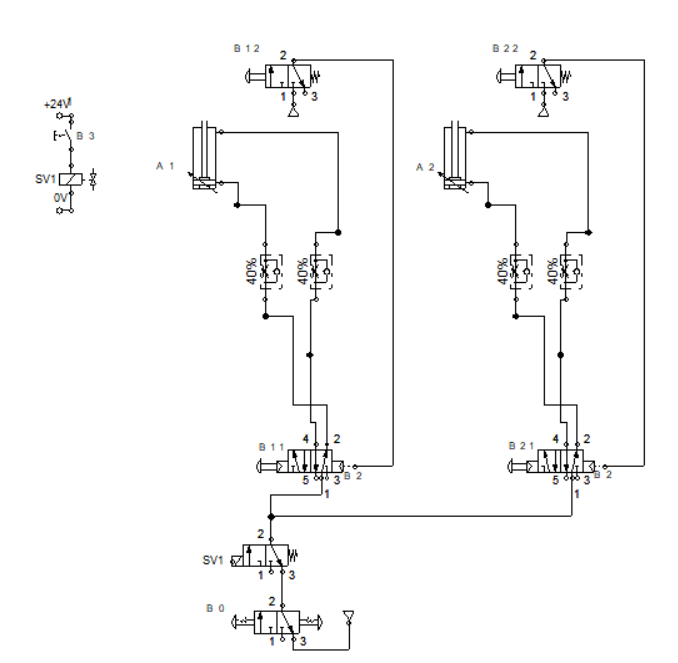
\includegraphics[width=16cm]{Images/Q4/fluidsim.png}
    \centering
    \caption{Fluidsim of the double elevator}
    \label{fig:fluidsim}
\end{figure}

\subsection{Conclusion}

This report details the complete development of an electropneumatic control system, from schematic 
design to simulation validation. By integrating various automation components and methodologies, 
the system achieves a robust and efficient control mechanism. The findings highlight the importance 
of precise component selection and control logic design in achieving a functional and reliable 
automated process.